\chapter{Metals: Reactions with Acids and Corrosion}\label{ch:g9:metals-acids-corrosion}

In a harbour, the steel hull of an old fishing boat is streaked with
orange \omterm{def:g9:metals-acids-corrosion:corrosion}{rust}. On the quay, a zinc-coated gate has stood in the rain for
thirty years and still shines dull grey. In a museum, a gold ring buried
for three thousand years is as bright as the day it was made. Metals do
not all face the world in the same way: some are attacked by water, \omterm{def:g4:air-a-mixture-of-gases:air}{air}
and acids, others hardly at all.

\begin{recall}
\omterm{def:g9:ions:ion}{Ions} are charged \omterm{def:g7:atoms-and-molecules:atom}{atoms}; metals give \omterm{def:g9:ions:ion}{cations} such as \ce{Fe^{2+}},
\ce{Zn^{2+}}, \ce{Al^{3+}}, identified by \omterm{def:g9:ions:precipitate}{precipitation} tests
(\cref{ch:g9:ions}). An \omterm{def:g9:acids-bases-ph:acidic}{acidic solution} contains many \ce{H+(aq)} \omterm{def:g9:ions:ion}{ions}
(\cref{ch:g9:acids-bases-ph}). Hydrogen burns with a squeaky pop at the
mouth of a test tube (\cref{ch:g7:identifying-substances}).
\end{recall}

\begin{omfigure}
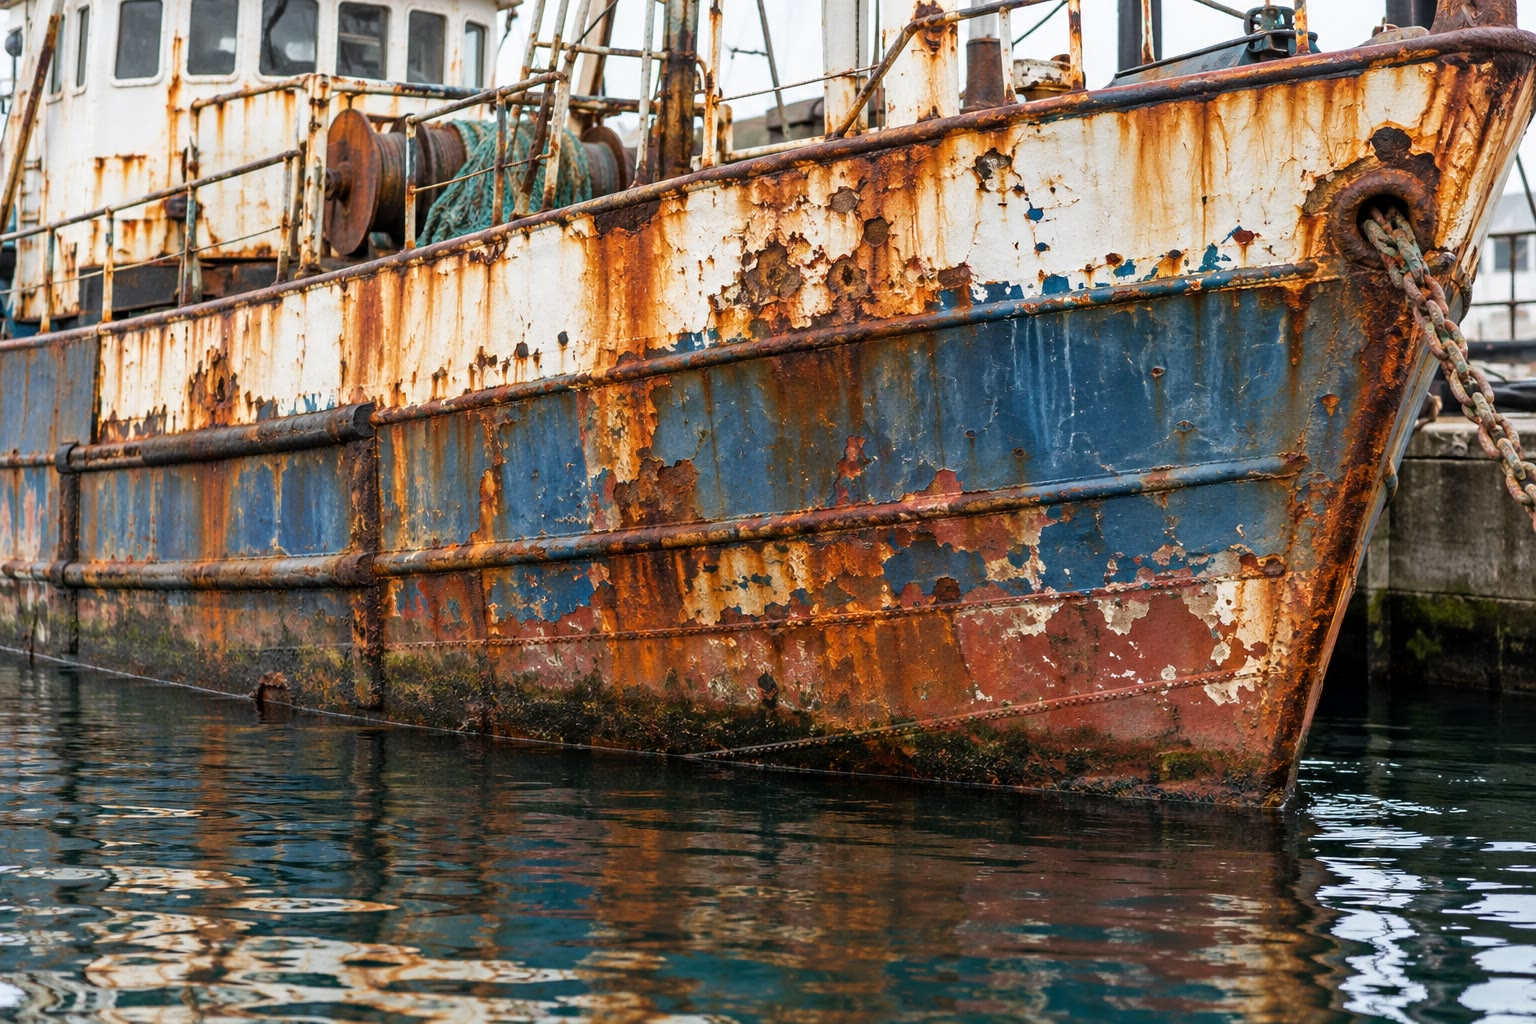
\includegraphics[width=0.55\linewidth]{images/book1/ai/g9-rusty-hull.jpg}

{\small The hull of an old boat: the steel is rusting.}
\end{omfigure}

\section{Metals in hydrochloric acid}

\begin{inthelab}[Three metals in acid]
The teacher drops a small piece of iron, of zinc and of copper into three
test tubes of dilute hydrochloric acid. Bubbles rise from the iron and the
zinc, slowly from the iron, briskly from the zinc, and the metals slowly
disappear; nothing happens to the copper. The gas, collected in a small
tube, gives a squeaky pop: it is hydrogen. With sodium hydroxide the
liquid of the first tube gives a green \omterm{def:g9:ions:precipitate}{precipitate} (\ce{Fe^{2+}} \omterm{def:g9:ions:ion}{ions}),
that of the second a white one (\ce{Zn^{2+}} \omterm{def:g9:ions:ion}{ions}).
\end{inthelab}

\begin{omfigure}
\begin{tikzpicture}[font=\small, scale=1.2]
  \foreach \k/\m/\c/\bub in {0/iron/black!45/4, 1/zinc/black!25/9, 2/copper/orange!60!brown/0} {
    \pic[transform shape] at (\k*2.4,0) {testtube={0.55}{omWater!70}};
    \fill[\c] (\k*2.4-0.13,0.08) rectangle (\k*2.4+0.13,0.35);
    \ifnum\bub>0
      \foreach \j in {1,...,\bub} {
        \pgfmathsetmacro\yy{0.45+0.12*\j}
        \pgfmathsetmacro\xx{\k*2.4+0.1*sin(97*\j)}
        \draw[black!55] (\xx,\yy) circle (0.035);
      }
    \fi
    \node[anchor=north, align=center] at (\k*2.4,-0.15) {\m};
  }
  \node[anchor=north, align=center, font=\footnotesize] at (0,-0.6) {bubbles, slowly};
  \node[anchor=north, align=center, font=\footnotesize] at (2.4,-0.6) {bubbles, briskly};
  \node[anchor=north, align=center, font=\footnotesize] at (4.8,-0.6) {no reaction};
\end{tikzpicture}

{\small Iron, zinc and copper in dilute hydrochloric acid: iron and zinc
give off hydrogen; copper does not react.}
\end{omfigure}

\begin{proposition}[Metal plus acid]\label{prop:g9:metals-acids-corrosion:acid}
Many metals --- iron, zinc, aluminium, magnesium --- react with the
\ce{H+} \omterm{def:g9:ions:ion}{ions} of an acid: the metal disappears as metal \omterm{def:g9:ions:ion}{ions}, which stay
dissolved, and hydrogen gas is given off. Copper, silver and gold do not
react with hydrochloric acid.
\end{proposition}

\section{Writing the equation with ions}

\begin{definition}[Spectator ion]\label{def:g9:metals-acids-corrosion:spectator}
An \omterm{def:g9:ions:ion}{ion} that is present in a solution during a reaction but takes no part
in it, and is found unchanged at the end, is a \emph{spectator
ion}\index{spectator ion}. It is left out of the equation.
\end{definition}

\begin{example}[Iron and zinc in hydrochloric acid]\label{ex:g9:metals-acids-corrosion:iron}
Hydrochloric acid contains \ce{H+(aq)} and \ce{Cl-(aq)} \omterm{def:g9:ions:ion}{ions}. The
chloride \omterm{def:g9:ions:ion}{ions} are found unchanged at the end: they are spectators. The
equations are
\[
  \ce{Fe(s) + 2H+(aq) -> Fe^{2+}(aq) + H2(g)}, \qquad
  \ce{Zn(s) + 2H+(aq) -> Zn^{2+}(aq) + H2(g)}.
\]
They balance both the \omterm{def:g7:atoms-and-molecules:atom}{atoms} and the charges: $+2$ on each side.
\end{example}

\begin{method}[Writing the equation of a metal with an acid]\label{met:g9:metals-acids-corrosion:write}
\begin{enumerate}
  \item \omterm{def:g7:chemical-reactions:reactant}{Reactants}: the metal (s) and the \ce{H+(aq)} \omterm{def:g9:ions:ion}{ions}.
  \item Products: the metal \omterm{def:g9:ions:ion}{ion} (aq), with its usual charge, and
        hydrogen \ce{H2(g)}.
  \item Balance the \omterm{def:g7:atoms-and-molecules:atom}{atoms}, then check that the total charge is the same
        on both sides.
\end{enumerate}
For aluminium: \ce{2Al(s) + 6H+(aq) -> 2Al^{3+}(aq) + 3H2(g)}; charge
$+6$ on each side.
\end{method}

\begin{safety}{\ghs[0.8cm]{GHS02}\ghs[0.8cm]{GHS04}}
% ledger: ghs:H2
The hydrogen given off is extremely flammable. The reaction is run in
small test tubes, by the teacher, far from any flame except the one used
for the pop test.
\end{safety}

\section{Corrosion}

\begin{definition}[Corrosion and rust]\label{def:g9:metals-acids-corrosion:corrosion}
\emph{Corrosion}\index{corrosion} is the slow attack of a metal by the
substances around it --- oxygen, water, acids, salts --- which turns the
metal into \omterm{def:g9:ions:ion}{ions} or into compounds such as oxides. The corrosion of iron
and steel produces \emph{rust}\index{rust}, a brown, crumbly, hydrated
iron oxide that flakes off and lets the attack go on deeper.
\end{definition}

\begin{proposition}[What iron needs to rust]\label{prop:g9:metals-acids-corrosion:needs}
Iron \omterm{def:g9:metals-acids-corrosion:corrosion}{rusts} only when both oxygen and water reach it. Salt dissolved in
the water, as on roads salted in winter or by the sea, makes rusting
faster.
\end{proposition}

\begin{inthelab}[Three nails, one week]
Three clean iron nails are placed in three test tubes: the first with
dry \omterm{def:g4:air-a-mixture-of-gases:air}{air} and a drying agent that removes water vapour; the second in
water boiled to remove its dissolved \omterm{def:g4:air-a-mixture-of-gases:air}{air}, covered with a layer of oil;
the third half in tap water, half in \omterm{def:g4:air-a-mixture-of-gases:air}{air}. After a week, only the third
nail is rusty.
\end{inthelab}

\begin{omfigure}
\begin{tikzpicture}[font=\small, scale=1.2]
  % tube 1: dry air, drying agent
  \pic[transform shape] at (0,0) {testtube={0.18}{white!80!black}};
  \foreach \x/\y in {-0.12/0.15,0.08/0.12,-0.02/0.3,0.12/0.32,-0.14/0.42,0.03/0.48}
    \fill[black!35] (\x,\y) circle (0.05);
  \fill[black!45] (-0.03,1.0) rectangle (0.03,2.4);
  \fill[black!45] (-0.09,2.4) rectangle (0.09,2.48);
  \fill[black!60] (-0.3,2.8) rectangle (0.3,3.1);
  \node[anchor=north, align=center] at (0,-0.15) {dry air:\\ no rust};
  % tube 2: boiled water under oil
  \pic[transform shape] at (2.6,0) {testtube={0.7}{omWater!80}};
  \fill[yellow!55!orange!60] (2.36,1.85) rectangle (2.84,2.1);
  \fill[black!45] (2.57,0.3) rectangle (2.63,1.7);
  \fill[black!45] (2.51,1.7) rectangle (2.69,1.78);
  \fill[black!60] (2.3,2.8) rectangle (2.9,3.1);
  \node[anchor=north, align=center] at (2.6,-0.15) {water without air:\\ no rust};
  % tube 3: water and air
  \pic[transform shape] at (5.2,0) {testtube={0.4}{omWater!80}};
  \fill[black!45] (5.17,0.3) rectangle (5.23,2.2);
  \fill[black!45] (5.11,2.2) rectangle (5.29,2.28);
  \fill[orange!60!brown] (5.15,0.9) rectangle (5.25,1.5);
  \node[anchor=north, align=center] at (5.2,-0.15) {water and air:\\ rust};
  \draw[<-, omProp, thick] (-0.15,0.3) -- (-0.9,0.7) node[left, text=black, font=\footnotesize] {drying agent};
  \draw[<-, omProp, thick] (2.85,1.98) -- (3.6,2.4) node[right, text=black, font=\footnotesize] {oil};
\end{tikzpicture}

{\small The three-nail experiment: iron \omterm{def:g9:metals-acids-corrosion:corrosion}{rusts} only where water and oxygen
reach it together, here at the surface of the water.}
\end{omfigure}

\begin{example}[Aluminium and copper protect themselves]\label{ex:g9:metals-acids-corrosion:protect}
Aluminium is attacked by the oxygen of the \omterm{def:g4:air-a-mixture-of-gases:air}{air} at once, but the thin
layer of oxide formed sticks to the metal and seals it from the \omterm{def:g4:air-a-mixture-of-gases:air}{air}:
aluminium window frames last for decades. Copper, slowly attacked by
\omterm{def:g4:air-a-mixture-of-gases:air}{air}, water and carbon dioxide, becomes covered with a green crust, the
patina, which also sticks and protects the metal below. \omterm{def:g9:metals-acids-corrosion:corrosion}{Rust}, by
contrast, flakes off.
\end{example}

\begin{omfigure}
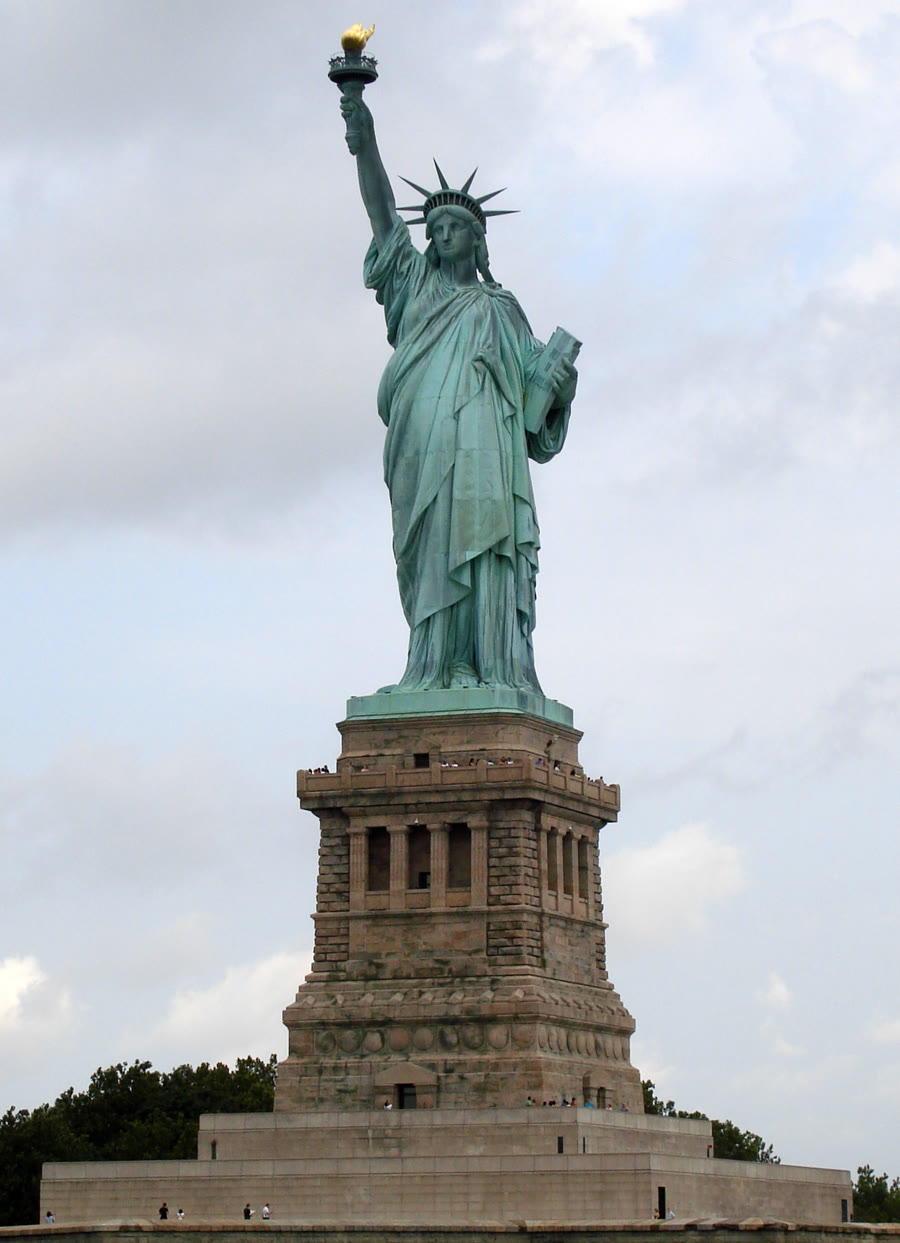
\includegraphics[height=6cm]{images/book1/statue-patina.jpg}

{\small The Statue of Liberty: its copper skin is covered with a green
patina. Photo: Elcobbola, public domain.}
\end{omfigure}

\section{Protecting metals}

\begin{definition}[Galvanising]\label{def:g9:metals-acids-corrosion:galvanising}
\emph{Galvanising}\index{galvanising} is coating steel with a layer of
zinc, by dipping it in molten zinc. Zinc is attacked by \omterm{def:g4:air-a-mixture-of-gases:air}{air} and water
rather than the steel below it: even where the coating is scratched, the
nearby zinc is corroded first and the steel is spared.
\end{definition}

\begin{proposition}[Ways to protect iron and steel]\label{prop:g9:metals-acids-corrosion:ways}
\begin{itemize}
  \item keep water and \omterm{def:g4:air-a-mixture-of-gases:air}{air} away: paint, oil, grease, a \omterm{def:g8:plastics:plastic}{plastic} coating;
  \item galvanise: a zinc layer that corrodes in place of the steel;
  \item use stainless steel, an alloy of iron with chromium, which
        protects itself with a thin sealing oxide layer;
  \item fix blocks of zinc to ship hulls: the zinc is slowly eaten away
        instead of the steel, and is replaced from time to time (how this
        works is explained in a university volume).
\end{itemize}
\end{proposition}

\begin{omfigure}
\begin{minipage}[b]{0.52\linewidth}\centering
\begin{tikzpicture}[font=\small]
  \fill[black!35] (0,0) rectangle (5,0.8);
  \fill[black!15] (0,0.8) rectangle (2.2,1.1);
  \fill[black!15] (2.8,0.8) rectangle (5,1.1);
  \fill[omWater!80] (1.6,1.1) rectangle (3.4,1.35);
  \fill[omWater!80] (2.2,0.8) rectangle (2.8,1.1);
  \draw[black!60] (0,0) rectangle (5,0.8);
  \foreach \x in {1.95,2.1} \draw[->, omProp, thick] (\x,1.25) -- (\x+0.05,1.7);
  \node[anchor=west, font=\footnotesize] at (5.1,0.4) {steel};
  \node[anchor=west, font=\footnotesize] at (5.1,0.95) {zinc layer};
  \node[anchor=south, font=\footnotesize, align=center] at (2.0,1.75) {zinc ions\\ go into the water};
  \node[anchor=north, font=\footnotesize, align=center] at (2.5,-0.05) {a scratch: the steel\\ is laid bare, but the zinc\\ around it corrodes first};
\end{tikzpicture}

{\small A scratched galvanised sheet.}
\end{minipage}\hfill
\begin{minipage}[b]{0.44\linewidth}\centering
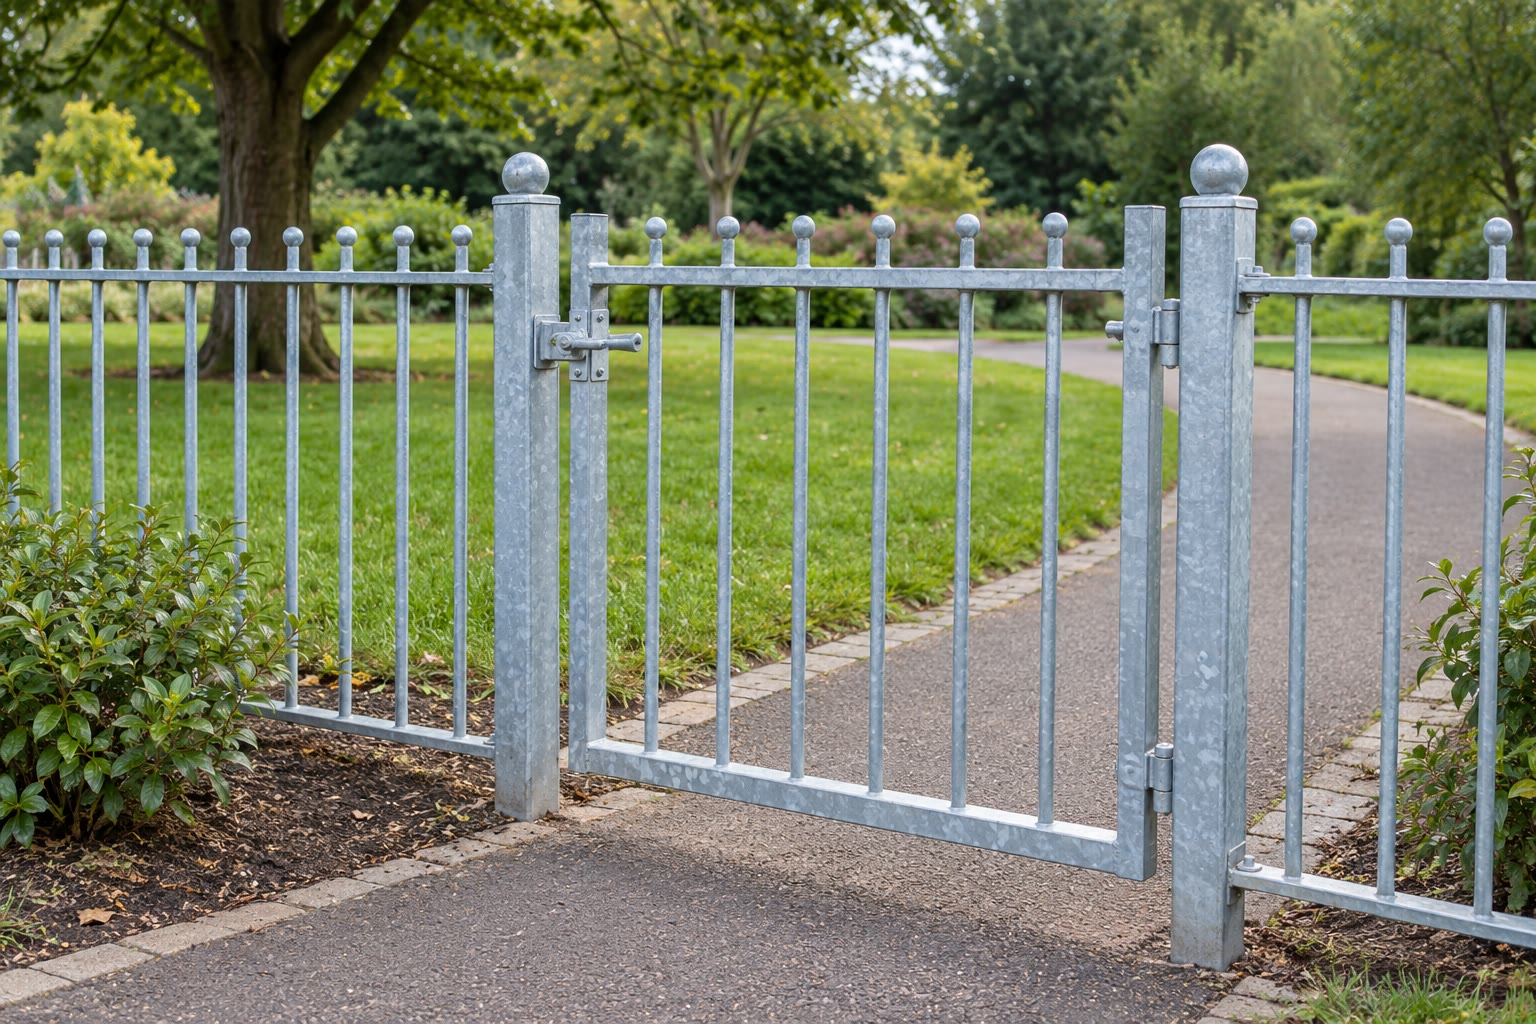
\includegraphics[width=\linewidth,height=4.4cm,keepaspectratio]{images/book1/ai/g9-galvanised-railings.jpg}

{\small Galvanised steel railings.}
\end{minipage}
\end{omfigure}

\section{Exercises}

\begin{exercise}[$\star$]\label{exo:g9:metals-acids-corrosion:1}
Which gas is given off when zinc reacts with hydrochloric acid? How is it
identified?
\end{exercise}

\begin{exercise}[$\star$]\label{exo:g9:metals-acids-corrosion:2}
Which of these metals react with dilute hydrochloric acid: iron, copper,
zinc, gold, aluminium?
\end{exercise}

\begin{exercise}[$\star$]\label{exo:g9:metals-acids-corrosion:3}
What does iron need in order to \omterm{def:g9:metals-acids-corrosion:corrosion}{rust}?
\end{exercise}

\begin{exercise}[$\star$]\label{exo:g9:metals-acids-corrosion:4}
What is a \omterm{def:g9:metals-acids-corrosion:spectator}{spectator ion}? Name the \omterm{def:g9:metals-acids-corrosion:spectator}{spectator ion} when iron reacts with
hydrochloric acid.
\end{exercise}

\begin{exercise}[$\star\star$]\label{exo:g9:metals-acids-corrosion:5}
Write the equation of the reaction of magnesium with the \ce{H+} \omterm{def:g9:ions:ion}{ions} of
an acid (the magnesium \omterm{def:g9:ions:ion}{ion} is \ce{Mg^{2+}}). Check the charges.
\end{exercise}

\begin{exercise}[$\star\star$]\label{exo:g9:metals-acids-corrosion:6}
After iron has reacted with hydrochloric acid, how can you show that the
solution contains iron(II) \omterm{def:g9:ions:ion}{ions}?
\end{exercise}

\begin{exercise}[$\star\star$]\label{exo:g9:metals-acids-corrosion:7}
Look at the three-nail figure. Why is the water of the second tube
boiled and covered with oil?
\end{exercise}

\begin{exercise}[$\star\star$]\label{exo:g9:metals-acids-corrosion:8}
Why does a car \omterm{def:g9:metals-acids-corrosion:corrosion}{rust} faster in a town where roads are salted in winter?
\end{exercise}

\begin{exercise}[$\star\star$]\label{exo:g9:metals-acids-corrosion:9}
Why do aluminium window frames not \omterm{def:g9:metals-acids-corrosion:corrosion}{rust} away, although aluminium reacts
with the oxygen of the \omterm{def:g4:air-a-mixture-of-gases:air}{air}?
\end{exercise}

\begin{exercise}[$\star\star$]\label{exo:g9:metals-acids-corrosion:10}
Give three ways of protecting a steel bicycle frame from \omterm{def:g9:metals-acids-corrosion:corrosion}{rust}.
\end{exercise}

\begin{exercise}[$\star\star\star$]\label{exo:g9:metals-acids-corrosion:11}
Write and check the equation of the reaction of aluminium with the
\ce{H+} \omterm{def:g9:ions:ion}{ions} of an acid. How many hydrogen \omterm{def:g7:atoms-and-molecules:molecule}{molecules} are formed for 200
aluminium \omterm{def:g7:atoms-and-molecules:atom}{atoms}?
\end{exercise}

\begin{exercise}[$\star\star\star$]\label{exo:g9:metals-acids-corrosion:12}
A galvanised steel bucket is scratched to the steel. Explain why the
steel at the bottom of the scratch does not \omterm{def:g9:metals-acids-corrosion:corrosion}{rust} for a long time.
\end{exercise}

\section{Problem: How Thick Is the Zinc?}

\begin{problem}[{Weekend problem --- dissolving the zinc coat of a
galvanised plate to find out how thick it was}]
\label{pb:g9:metals-acids-corrosion:1}
% ledger: rho:Zn
A galvanised steel plate, a square of side \qty{10.0}{cm}, is coated with
zinc on both faces (the edges are neglected). In a laboratory, the teacher
weighs it, \qty{125.6}{g}, then dips it in hydrochloric acid containing an
additive that stops the acid from attacking the steel. When the bubbling
stops, the plate is rinsed, dried and weighed again: \qty{113.5}{g}. The
mass of \qty{1}{cm^3} of zinc is \qty{7.13}{g}.

\medskip
\noindent\textbf{Part I --- The reaction.}
\begin{enumerate}
  \item Write the equation of the reaction of zinc with the \ce{H+} \omterm{def:g9:ions:ion}{ions}
        of the acid.
  \item Which gas causes the bubbling? Describe its test.
  \item Which test would show the zinc \omterm{def:g9:ions:ion}{ions} in the solution afterwards?
  \item Name the \omterm{def:g9:metals-acids-corrosion:spectator}{spectator ions}.
\end{enumerate}

\medskip
\noindent\textbf{Part II --- The zinc.}
\begin{enumerate}[resume]
  \item What mass of zinc has dissolved?
  \item Why is the bubbling a sign that the zinc has not all been
        dissolved yet?
  \item What would happen to the steel if the acid did not contain the
        additive? Which test would then show it?
  \item Why does the zinc protect the steel of the plate as long as it is
        there?
\end{enumerate}

\medskip
\noindent\textbf{Part III --- The thickness.}
\begin{enumerate}[resume]
  \item What is the total coated area of the plate, in \unit{cm^2}?
  \item What volume did the zinc occupy?
  \item Deduce the thickness of the zinc layer, in centimetres.
  \item Express this thickness in micrometres
        (\qty{1}{cm} $= \qty{10000}{\micro m}$).
\end{enumerate}
\end{problem}
